\section{Experiments}
\label{sec:experiments}

We comprehensively evaluate JuZhou 1.0 from both quantitative and qualitative perspectives. The quantitative evaluation measures semantic alignment on the GenEval benchmark against mainstream English-centric baselines (SDv2.1 and SDXL), while the qualitative evaluation examines foundational generation fidelity, distillation efficacy, and native Chinese cultural alignment through systematic visual comparisons. Unless otherwise noted, all GenEval evaluations use the 28-step base model for fair comparison, and all on-device latency measurements use the 4-step distilled model.

\subsection{Experimental Setup}
\label{sec:experimentalSetup}
We adopt a progressive resolution scaling strategy to enable a smooth transition from low- to high-resolution synthesis. 
% The training pipeline consists of two stages: 28-step foundational training and 4-step accelerated distillation. During foundational training, the model is sequentially trained at $256\times256$, $512\times512$, and $1024\times1024$ resolutions. The subsequent 4-step distillation at $1024\times1024$ significantly improves inference efficiency while preserving generation fidelity.
The training pipeline consists of two phases and three reported stages. The first phase is 28-step foundational training, which includes Stage 1 low-resolution pre-training at $256\times256$ and Stage 2 progressive-resolution training from $512\times512$ to $1024\times1024$. The second phase is Stage 3 DMD2-based step compression, which distills the 28-step model into a 4-step model at $1024\times1024$.

% All training and distillation experiments are conducted on a Sugon K100 AI cluster with 60 compute nodes and 240 K100 DCUs. 
All model training and distillation experiments were conducted on the Sugon K100 AI cluster, with stage-specific resource allocation. The low-resolution pre-training and progressive-resolution foundational training stages used 56 compute nodes with 224 K100 DCUs, while the DMD2 step-compression stage used 40 compute nodes with 160 K100 DCUs.
Quantitative evaluation and baseline comparison are performed in a unified NVIDIA V100 environment, while on-device latency is measured on the target mobile devices.

For quantitative evaluation on the GenEval benchmark, we use our 28-step English base model to ensure a fair comparison with established English-centric baselines, including Stable Diffusion v2.1 (SDv2.1) and SDXL. The detailed configuration of each training stage is reported in Tab.~\ref{tab:training_config}, including resolution, dataset, cluster scale, global batch size, training steps, learning rate, and optimizer settings.


% \begin{table}[t]
%     \centering
%     \caption{Training configuration for each stage of the JuZhou 1.0 multi-stage training framework. All stages are conducted on the Sugon K100 AI cluster. (BS: Global Batch Size, LR: Learning Rate, Opt.: Optimizer)}
%     \label{tab:training_config}
%     \small
%     \setlength{\tabcolsep}{1pt}
%     \renewcommand{\arraystretch}{1.15}
%     \begin{tabular}{lccccccc}
%         \toprule
%         \textbf{Stage} 
%         & \textbf{Resolution} 
%         & \textbf{Data} 
%         & \textbf{Nodes$\times$DCUs}
%         & \textbf{BS}
%         & \textbf{Steps} 
%         & \textbf{LR}
%         & \textbf{Opt.} \\
%         \midrule
%         1: Low-Res Pre-training 
%         & $256\times256$ 
%         & ImageNet-1K 
%         & $56 \times 4$ 
%         & 114{,}688 
%         & 30K 
%         & $3 \times 10^{-4}$ 
%         & AdamW \\
%         2: Progressive Resolution 
%         & $512{\to}1024$ 
%         & 9M Chinese pairs 
%         & $56 \times 4$ 
%         & 2{,}688 
%         & 150K 
%         & $1 \times 10^{-4}$ 
%         & AdamW \\
%         3: Step Compression (DMD2) 
%         & $1024\times1024$ 
%         & 9M Chinese pairs 
%         & $40 \times 4$ 
%         & 960 
%         & 10K 
%         & $1 \times 10^{-5}$ 
%         & AdamW \\
%         \bottomrule
%     \end{tabular}
%     \renewcommand{\arraystretch}{1.0}
%     \setlength{\tabcolsep}{6pt}
% \end{table}
\begin{table}[t]
    \centering
    \caption{Training configuration for each stage of the JuZhou 1.0 multi-stage training framework. All stages are conducted on the Sugon K100 AI cluster. (BS: Global Batch Size, LR: Learning Rate, Opt.: Optimizer)}
    \label{tab:training_config}
    \small
    \setlength{\tabcolsep}{5pt}
    \renewcommand{\arraystretch}{1.15}

    \resizebox{\linewidth}{!}{
    \begin{tabular}{@{}lccccccc@{}}
        \toprule
        \textbf{Stage} 
        & \textbf{Resolution} 
        & \textbf{Data} 
        & \textbf{Nodes $\times$ DCUs}
        & \textbf{BS}
        & \textbf{Steps} 
        & \textbf{LR}
        & \textbf{Opt.} \\
        \midrule
        1: Low-Res Pre-training 
        & $256\times256$ 
        & ImageNet-1K 
        & $56 \times 4$ 
        & 114{,}688 
        & 30K 
        & $3 \times 10^{-4}$ 
        & AdamW \\
        2: Progressive Resolution 
        & $512{\to}1024$ 
        & 9M Chinese pairs 
        & $56 \times 4$ 
        & 2{,}688 
        & 150K 
        & $1 \times 10^{-4}$ 
        & AdamW \\
        3: Step Compression (DMD2) 
        & $1024\times1024$ 
        & 9M Chinese pairs 
        & $40 \times 4$ 
        & 960 
        & 10K 
        & $1 \times 10^{-5}$ 
        & AdamW \\
        \bottomrule
    \end{tabular}
    }

    \renewcommand{\arraystretch}{1.0}
    \setlength{\tabcolsep}{6pt}
\end{table}

\subsection{Quantitative Results}

To evaluate the semantic understanding and compositional reasoning capabilities of the JuZhou~1.0 base model, we conduct a systematic evaluation on the GenEval benchmark~\cite{ghosh2023geneval}. GenEval measures fine-grained text-to-image alignment across several complementary dimensions, including object generation (\textit{Single} and \textit{Two}), numerical reasoning (\textit{Count}), attribute recognition (\textit{Color}), spatial reasoning (\textit{Position}), and attribute--object binding (\textit{Color Attr.}).

As shown in Tab.~\ref{tab:geneval_performance}, JuZhou~1.0 achieves an overall GenEval score of \textbf{0.69} with only \textbf{0.387B} denoising parameters. Among all evaluated models, this represents the second-highest overall score, surpassed only by FLUX.1-schnell at 0.71, while JuZhou~1.0 uses approximately $31\times$ fewer denoising parameters. It also substantially outperforms several larger server-oriented models, including SD3-Medium, SDXL, IF-XL, PlayGround~v2.5, Hunyuan-DiT, and both Sana variants. Compared with compact baselines, JuZhou~1.0 improves the overall score from 0.66 for SnapGen and Sana-1.6B to 0.69, while maintaining a highly compact model size. With 0.387B parameters, JuZhou~1.0 is the second-smallest model in the comparison, only slightly larger than the 0.373B SnapGen.

These results are obtained under a substantially constrained deployment setting. JuZhou~1.0 is trained end-to-end on a China-developed accelerator stack and is explicitly designed for offline execution on mobile devices. In contrast, most evaluated baselines contain substantially more parameters and are primarily intended for server-side inference. Among the models listed in Tab.~\ref{tab:geneval_performance}, only JuZhou~1.0 and SnapGen support mobile deployment, while JuZhou~1.0 achieves a notably higher overall GenEval score.

A closer examination of the category-level results further demonstrates that the compact architecture preserves strong compositional and attribute-binding capabilities. JuZhou~1.0 achieves a \textit{Two} score of \underline{0.87}, ranking second among all evaluated models and trailing only FLUX.1-schnell. It also obtains a \textit{Color} score of \textbf{0.88}, tied for the best performance, and a \textit{Color Attr.} score of \textbf{0.55}, which is the highest score in the comparison. These results indicate that JuZhou~1.0 can reliably generate multiple objects with specified visual attributes and associate colors with the corresponding objects despite its highly compressed denoising network. In addition, its \textit{Position} score of 0.24 ranks third overall, outperforming all compact and efficient baselines included in the comparison.

JuZhou~1.0 nevertheless exhibits limitations in numerical reasoning. Its \textit{Count} score of 0.61 remains below those of several larger models, such as FLUX.1-dev, FLUX.1-schnell, Hunyuan-DiT, and IF-XL. This suggests that accurately representing object multiplicity remains challenging under strict model-capacity constraints and constitutes an important direction for future improvement. The \textit{Single} score of 0.99 is also highly competitive, although several models already approach saturation on this relatively simple category.

% Overall, the significance of these results lies not only in the absolute GenEval score, but also in the model scale and deployment context under which it is achieved. JuZhou~1.0 combines the second-highest overall GenEval performance in the comparison with only 0.387B denoising parameters and practical offline mobile deployment. The results demonstrate that a compact text-to-image foundation model trained on a domestic accelerator stack can retain competitive semantic alignment, compositional reasoning, and fine-grained attribute binding without relying on conventional server-scale architectures. Together with the on-device deployment results, this favorable balance between generation quality, model compactness, and deployment efficiency establishes JuZhou~1.0 as a viable solution for edge-native text-to-image generation.
Overall, JuZhou~1.0 achieves a strong balance between GenEval performance, compact model scale, and practical offline deployment. With a 0.387B image-generation backbone, it attains the second-highest overall GenEval score in the comparison while supporting on-device inference. These results suggest that compact T2I models trained on domestic accelerator stacks can retain competitive semantic alignment and compositional ability without relying on server-scale architectures.

\begin{table}[t]
    \centering
    % \caption{Quantitative evaluation on the GenEval benchmark. All models are evaluated at $1024 \times 1024$ resolution. Params and overall score are placed side by side to highlight the performance--parameter trade-off. JuZhou~1.0 achieves an overall score of 0.69 with only 0.385B parameters, matching Hunyuan-DiT while using about $3.75\times$ fewer parameters, and outperforming SD3-Medium and IF-XL despite a substantially smaller model size.}
    \caption{Quantitative evaluation on the GenEval benchmark. All models are evaluated at $1024 \times 1024$ resolution. Params and overall score are placed side by side to highlight the performance--parameter trade-off. The ``Mobile'' column indicates whether a model has reported or validated smartphone-side image-generation deployment, rather than merely compact parameter count. JuZhou~1.0 achieves an overall score of 0.69 with a 0.387B-parameter image-generation backbone, showing a favorable accuracy--efficiency trade-off compared with larger baselines such as Hunyuan-DiT, SD3-Medium, and IF-XL.}
    \label{tab:geneval_performance}
    \resizebox{\textwidth}{!}{%

    \begin{tabular}{lccccccccc}
        \toprule
        \textbf{Method} 
        & \textbf{Params$\downarrow$} 
        & \textbf{Overall$\uparrow$} 
        & \textbf{Mobile} 
        & \textbf{Single$\uparrow$} 
        & \textbf{Two$\uparrow$} 
        & \textbf{Count$\uparrow$} 
        & \textbf{Color$\uparrow$} 
        & \textbf{Pos.$\uparrow$} 
        & \textbf{Color Attr.$\uparrow$} \\
        \midrule
        \midrule
    
        \multicolumn{10}{l}{\textit{Large-scale baselines}} \\
        \midrule
    
        LUMINA-Next~\cite{zhuo2024luminanext}
        & 2.0B
        & 0.46
        & {\color{red}\ding{55}}
        & 0.92
        & 0.46
        & 0.48
        & 0.70
        & 0.09
        & 0.13 \\
    
        SD3-Medium~\cite{esser2024scaling}
        & 2.0B
        & 0.62
        & {\color{red}\ding{55}}
        & \textit{0.98}
        & 0.74
        & 0.63
        & 0.67
        & \textbf{0.34}
        & 0.36 \\
    
        SDXL~\cite{podell2023sdxl}
        & 2.6B
        & 0.55
        & {\color{red}\ding{55}}
        & \textit{0.98}
        & 0.74
        & 0.39
        & \underline{0.85}
        & 0.15
        & 0.23 \\
    
        PlayGround v2.5~\cite{li2024playgroundv25}
        & 2.6B
        & 0.56
        & {\color{red}\ding{55}}
        & \textit{0.98}
        & 0.77
        & 0.52
        & \textit{0.84}
        & 0.11
        & 0.17 \\
    
        IF-XL~\cite{deepfloyd2023if}
        & 4.3B
        & 0.61
        & {\color{red}\ding{55}}
        & 0.97
        & 0.74
        & 0.66
        & 0.81
        & 0.13
        & 0.35 \\
    
        FLUX.1-dev~\cite{flux2024}
        & 12.0B
        & \textit{0.67}
        & {\color{red}\ding{55}}
        & \underline{0.99}
        & 0.81
        & \textbf{0.79}
        & 0.74
        & 0.20
        & \textit{0.47} \\
    
        FLUX.1-schnell~\cite{flux2024}
        & 12.0B
        & \textbf{0.71}
        & {\color{red}\ding{55}}
        & \underline{0.99}
        & \textbf{0.92}
        & \underline{0.73}
        & 0.78
        & \underline{0.28}
        & \underline{0.54} \\
    
        \midrule
        \multicolumn{10}{l}{\textit{Compact and efficient baselines}} \\
        \midrule
    
        SnapGen~\cite{hu2024snapgen}
        & \textbf{0.373B}
        & 0.66
        & {\color{green}\ding{51}}
        & \textbf{1.00}
        & \textit{0.84}
        & 0.60
        & \textbf{0.88}
        & 0.18
        & 0.45 \\
    
        Sana-0.6B~\cite{xie2024sana}
        & \textit{0.6B}
        & 0.64
        & {\color{red}\ding{55}}
        & \underline{0.99}
        & 0.76
        & 0.64
        & \textbf{0.88}
        & 0.18
        & 0.39 \\
    
        SDv2.1~\cite{stability2022sd21}
        & 1.3B
        & 0.50
        & {\color{red}\ding{55}}
        & \textit{0.98}
        & 0.51
        & 0.44
        & \underline{0.85}
        & 0.07
        & 0.17 \\
    
        Hunyuan-DiT~\cite{li2024hunyuandit}
        & 1.5B
        & 0.63
        & {\color{red}\ding{55}}
        & 0.97
        & 0.77
        & \textit{0.71}
        & \textbf{0.88}
        & 0.13
        & 0.30 \\
    
        Sana-1.6B~\cite{xie2024sana}
        & 1.6B
        & 0.66
        & {\color{red}\ding{55}}
        & \underline{0.99}
        & 0.77
        & 0.62
        & \textbf{0.88}
        & 0.21
        & \textit{0.47} \\
    
        \midrule
        \rowcolor{DeepTeal!15}
        \textbf{Ours}
        & \underline{0.387B}
        & \underline{0.69}
        & {\color{green}\ding{51}}
        & \underline{0.99}
        & \underline{0.87}
        & 0.61
        & \textbf{0.88}
        & \textit{0.24}
        & \textbf{0.55} \\
    
        \bottomrule
    \end{tabular}%

    }
\end{table}

\subsection{Qualitative Results}

We conduct qualitative evaluations along three complementary axes: foundational generation quality compared against the Stable Diffusion family, the efficacy of our 4-step distillation in preserving visual fidelity, and the model's capability to capture native Chinese cultural semantics through classical poetry generation.

\begin{figure}[htbp]
\centering
\small
\setlength{\tabcolsep}{2pt}
\begin{tabular}{ccccc}
\textbf{Ours (28 steps)} & \textbf{SD1.5 (40 steps)} & \textbf{SD2.1 (40 steps)} & \textbf{SDXL (40 steps)} & \textbf{SD3.5-L (28 steps)} \\

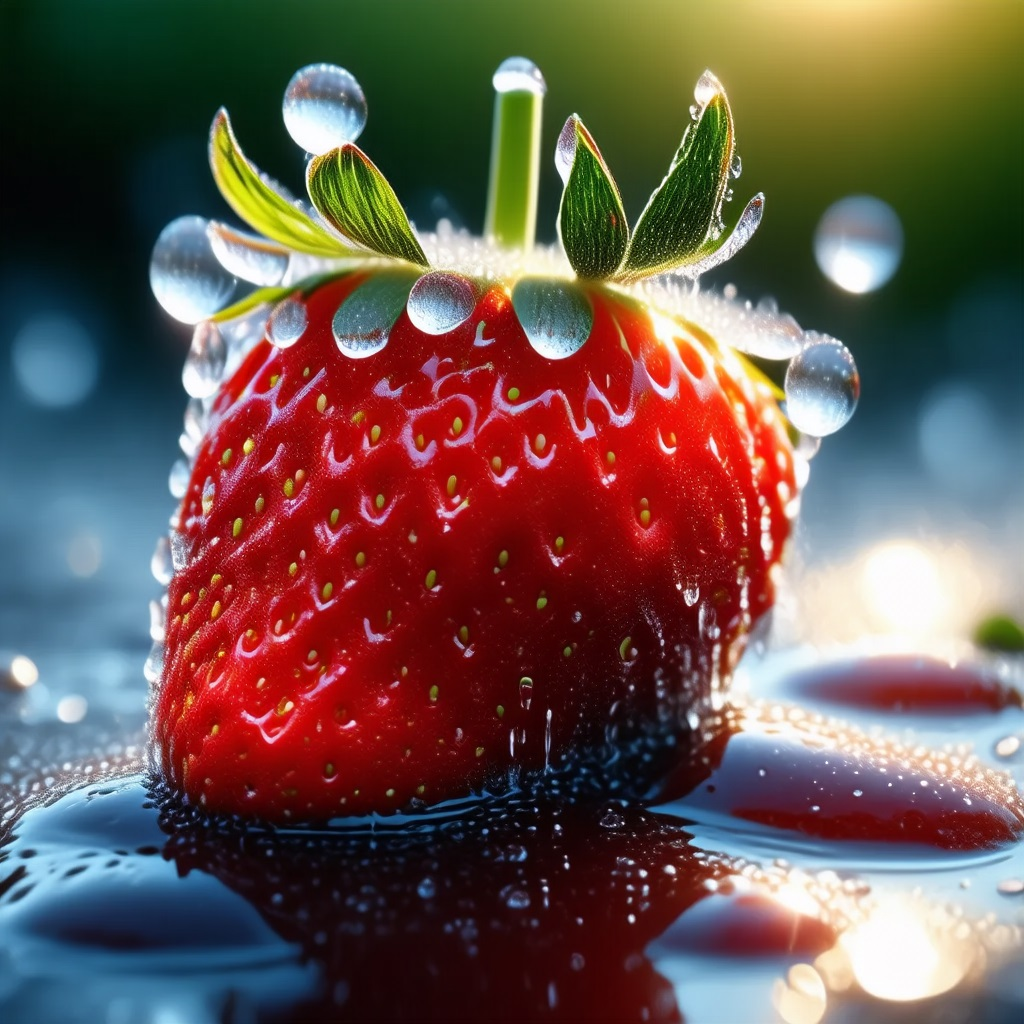
\includegraphics[width=0.19\linewidth]{figures/sec05_experiments/foundational_jz_fig/144000_jpg_prompt2_img2.jpg} &
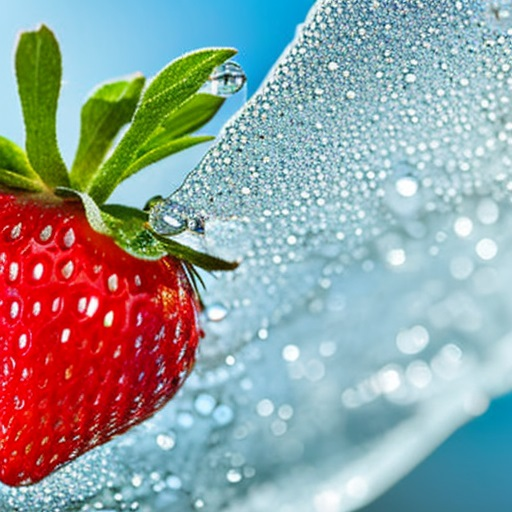
\includegraphics[width=0.19\linewidth]{figures/sec05_experiments/foundational_sd_fig/002_20260309_193620.jpg} &

\includegraphics[width=0.19\linewidth]{figures/sec05_experiments/SDV21/image_001.jpg} &

\includegraphics[width=0.19\linewidth]{figures/sec05_experiments/SDxl/image_001.jpg} &
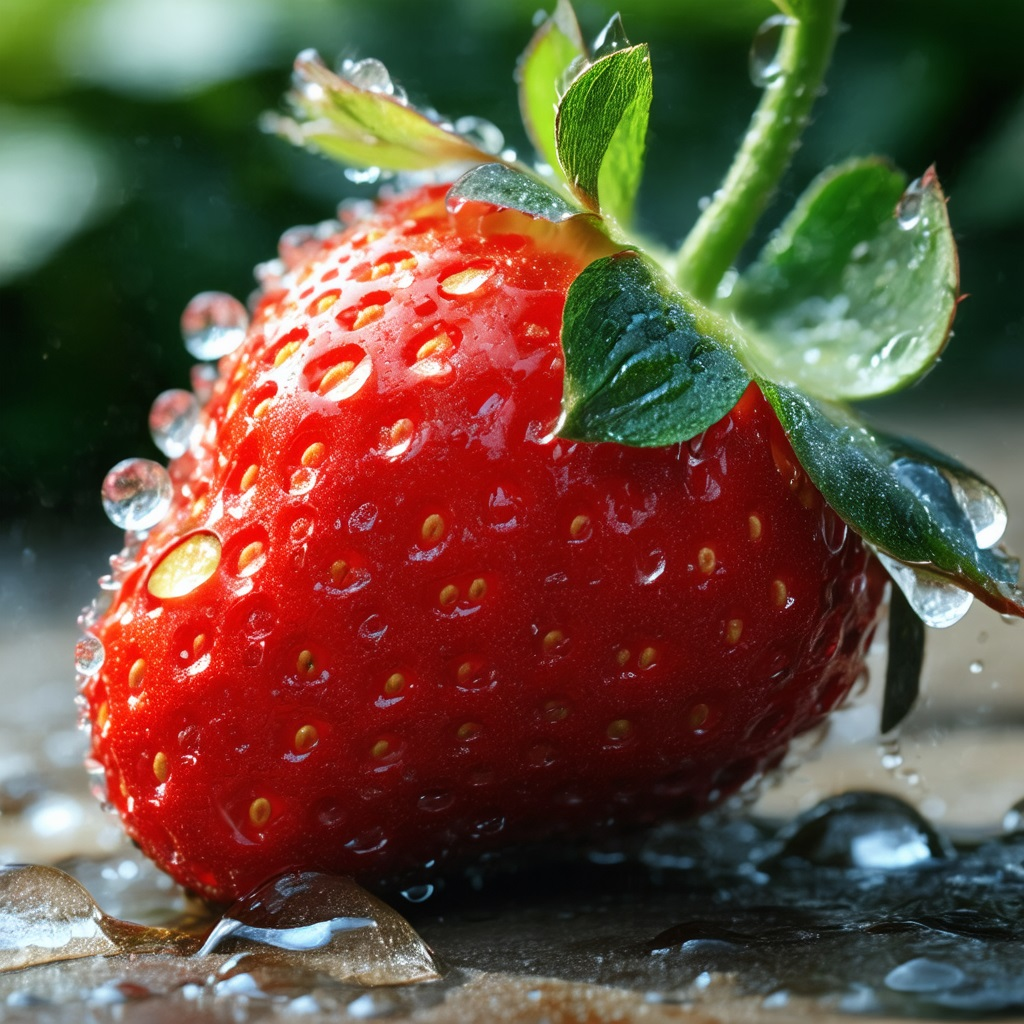
\includegraphics[width=0.19\linewidth]{figures/sec05_experiments/SD35/image_001.jpg} \\
\multicolumn{5}{p{0.98\linewidth}}{\centering\footnotesize (a) Macro shot of a dew-covered strawberry, crystal water droplets, soft morning sun, 8k resolution, photorealistic.} \\[1pt]

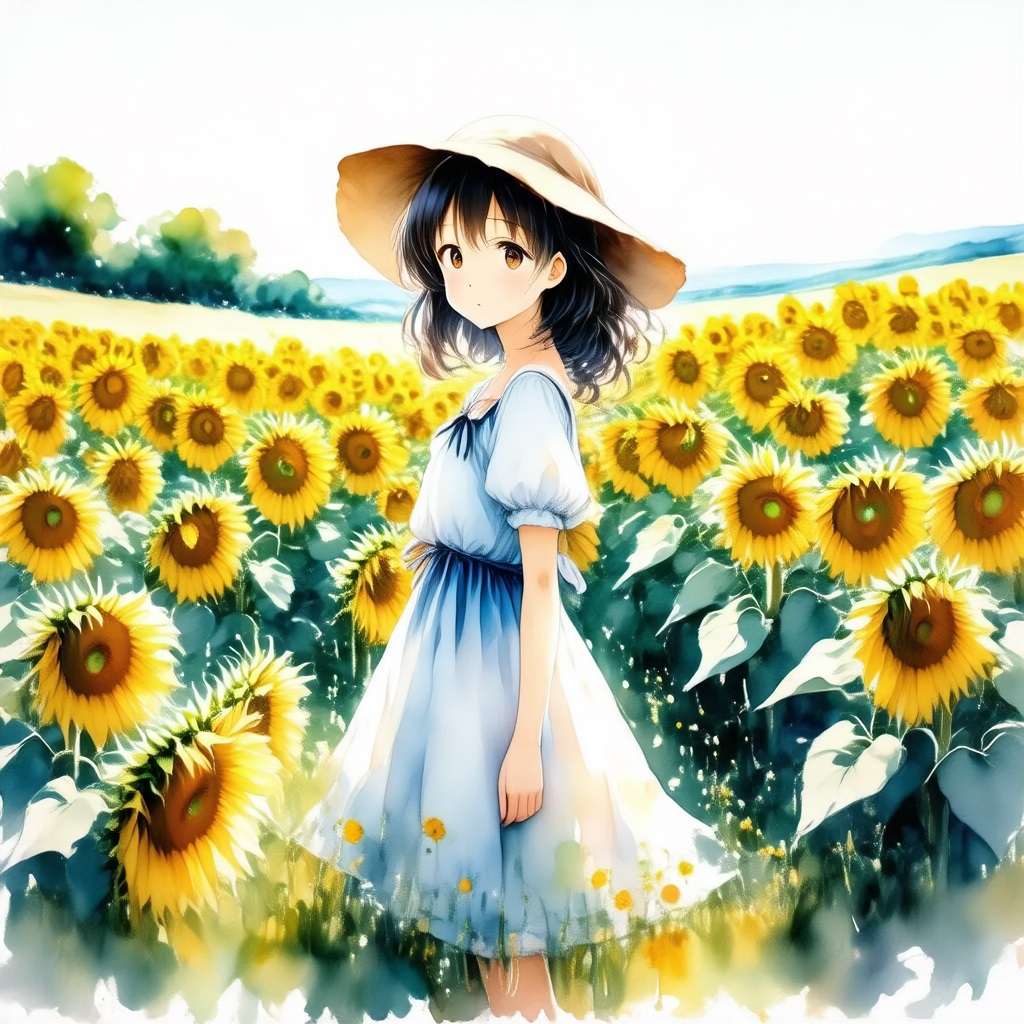
\includegraphics[width=0.19\linewidth]{figures/sec05_experiments/foundational_jz_fig/144000_jpg_prompt9_img1.jpg} &
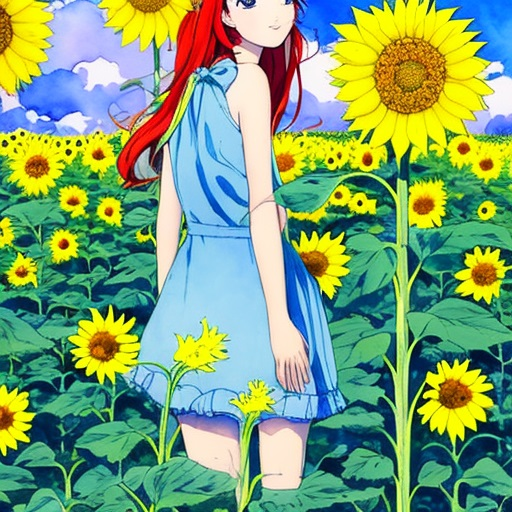
\includegraphics[width=0.19\linewidth]{figures/sec05_experiments/foundational_sd_fig/009_20260309_193638.jpg} &

\includegraphics[width=0.19\linewidth]{figures/sec05_experiments/SDV21/image_008.jpg} &

\includegraphics[width=0.19\linewidth]{figures/sec05_experiments/SDxl/image_008.jpg} &
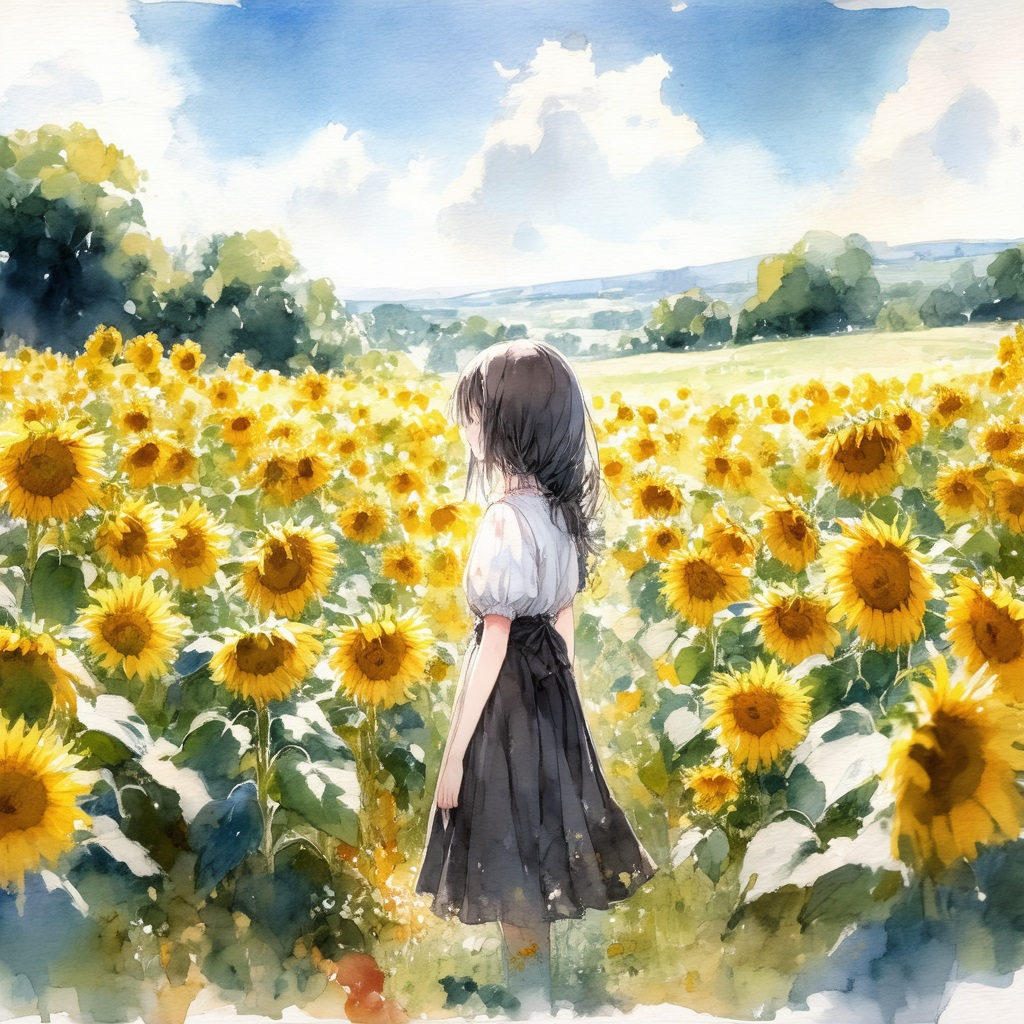
\includegraphics[width=0.19\linewidth]{figures/sec05_experiments/SD35/image_008.jpg} \\
\multicolumn{5}{p{0.98\linewidth}}{\centering\footnotesize (b) A beautiful anime girl standing in a field of sunflowers, soft watercolor anime style, hand-drawn animation aesthetics, dreamy mood.} \\[1pt]

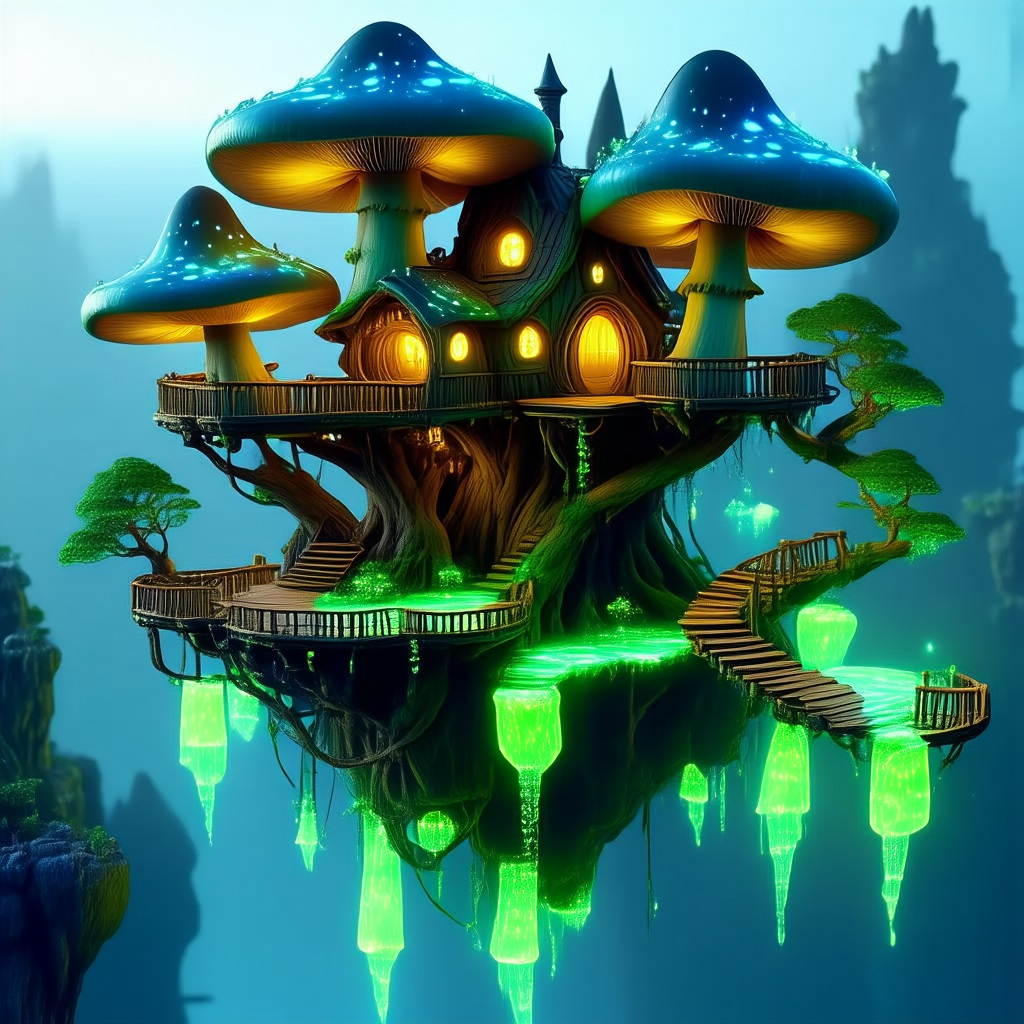
\includegraphics[width=0.19\linewidth]{figures/sec05_experiments/foundational_jz_fig/144000_jpg_prompt10_img3.jpg} &
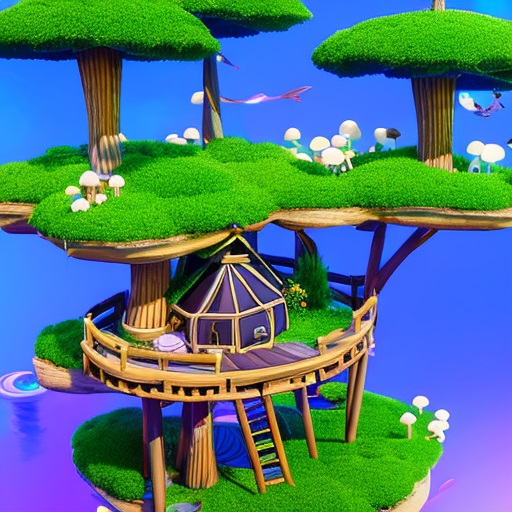
\includegraphics[width=0.19\linewidth]{figures/sec05_experiments/foundational_sd_fig/010_20260309_193640.jpg} &

\includegraphics[width=0.19\linewidth]{figures/sec05_experiments/SDV21/image_009.jpg} &

\includegraphics[width=0.19\linewidth]{figures/sec05_experiments/SDxl/image_009.jpg} &
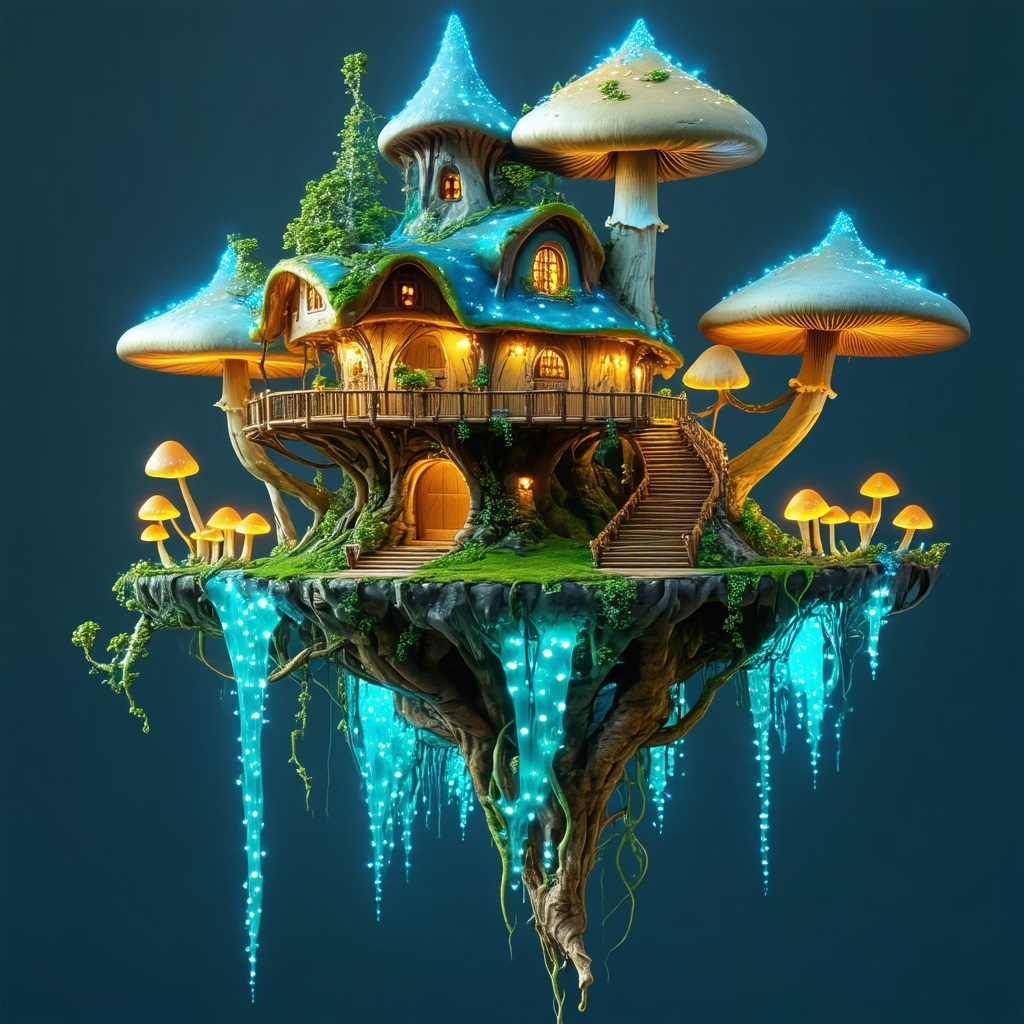
\includegraphics[width=0.19\linewidth]{figures/sec05_experiments/SD35/image_009.jpg} \\
\multicolumn{5}{p{0.98\linewidth}}{\centering\footnotesize (c) An isometric view of a magical floating treehouse, bioluminescent mushrooms, fantasy art, Unreal Engine 5 render.} \\[1pt]

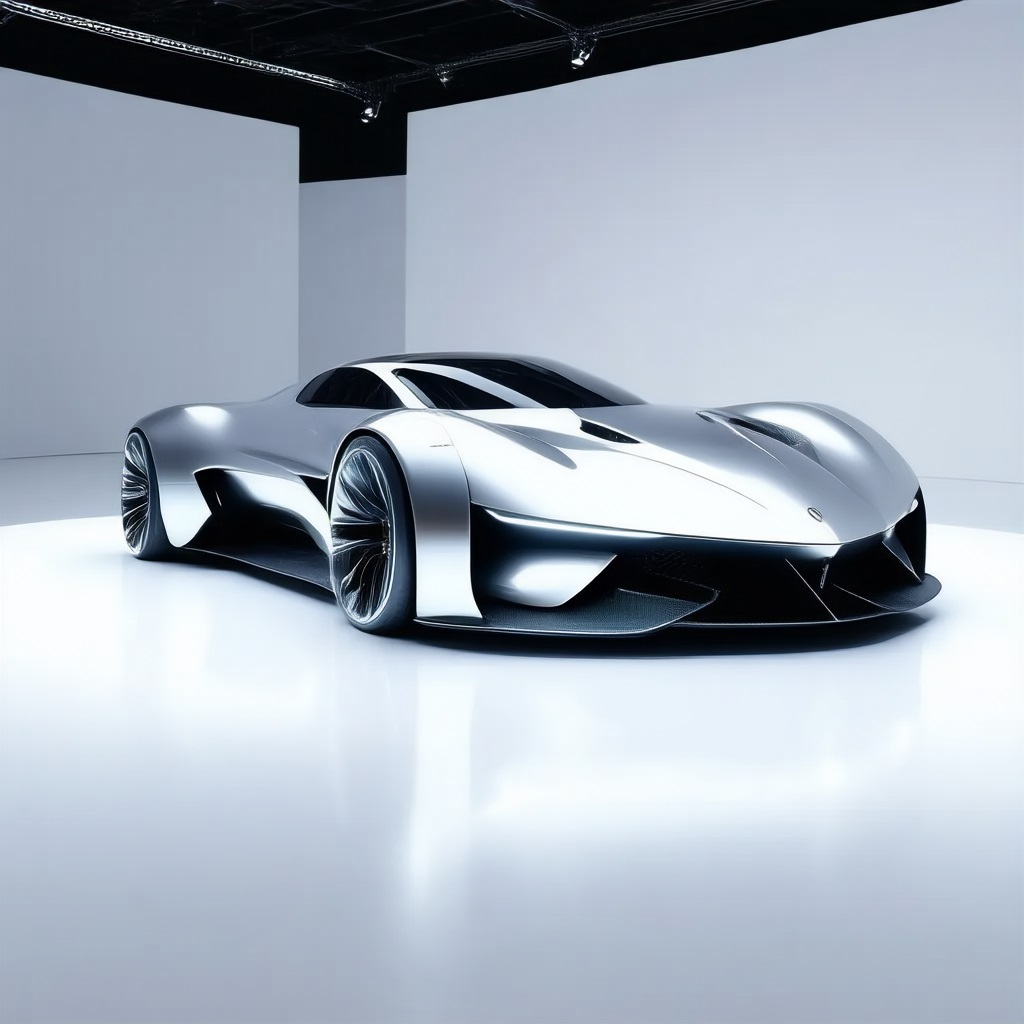
\includegraphics[width=0.19\linewidth]{figures/sec05_experiments/foundational_jz_fig/144000_jpg_prompt11_img4.jpg} &
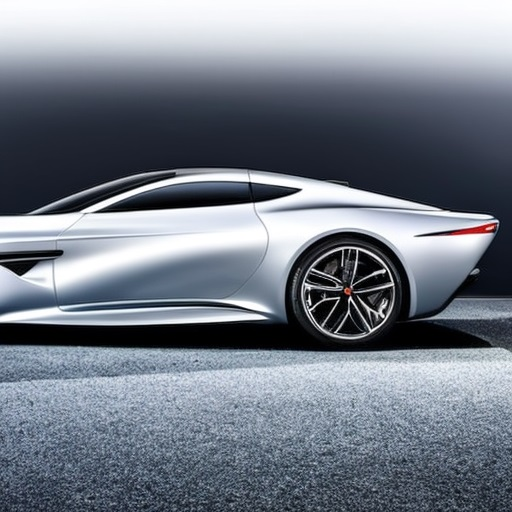
\includegraphics[width=0.19\linewidth]{figures/sec05_experiments/foundational_sd_fig/011_20260309_193643.jpg} &

\includegraphics[width=0.19\linewidth]{figures/sec05_experiments/SDV21/image_010.jpg} &

\includegraphics[width=0.19\linewidth]{figures/sec05_experiments/SDxl/image_010.jpg} &
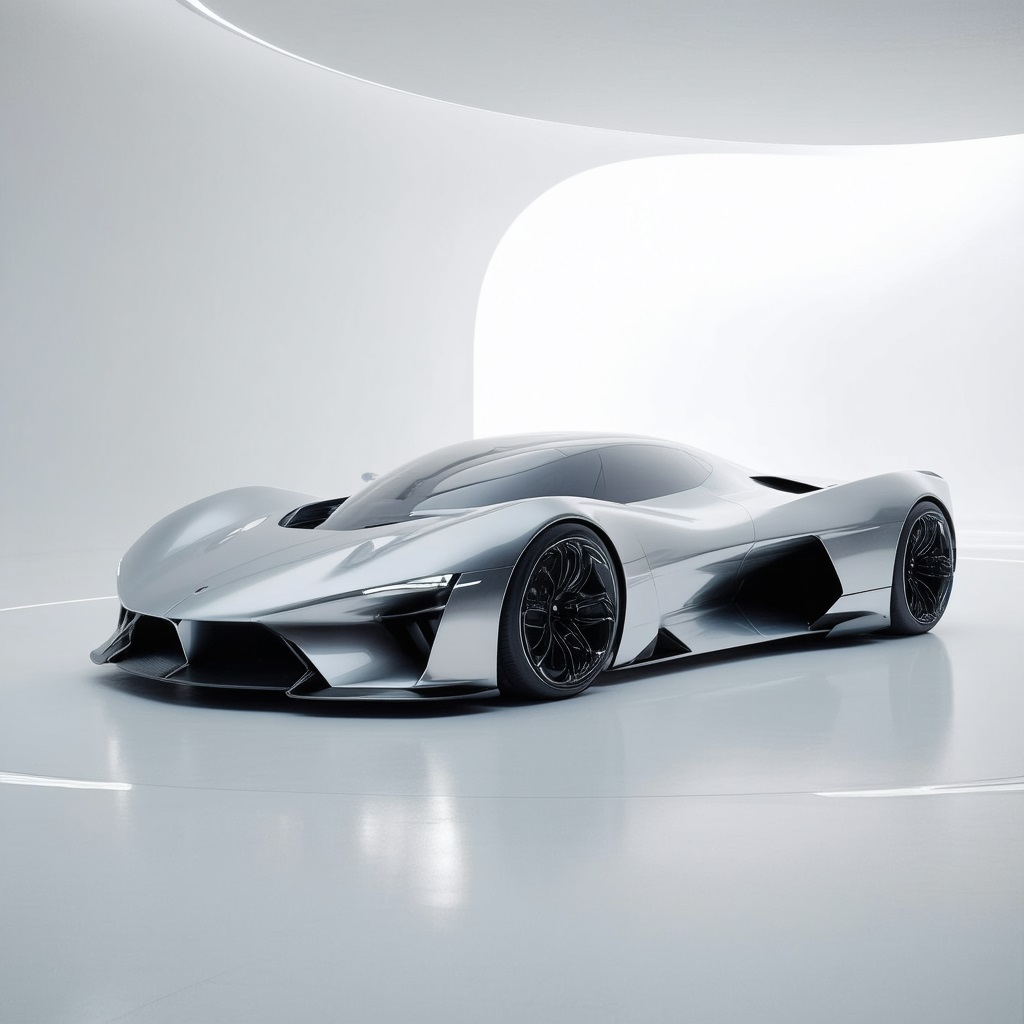
\includegraphics[width=0.19\linewidth]{figures/sec05_experiments/SD35/image_010.jpg} \\
\multicolumn{5}{p{0.98\linewidth}}{\centering\footnotesize (d) A futuristic sports car on a minimalist white stage, sleek silver body, bright studio spotlights, automotive photography.} \\[1pt]

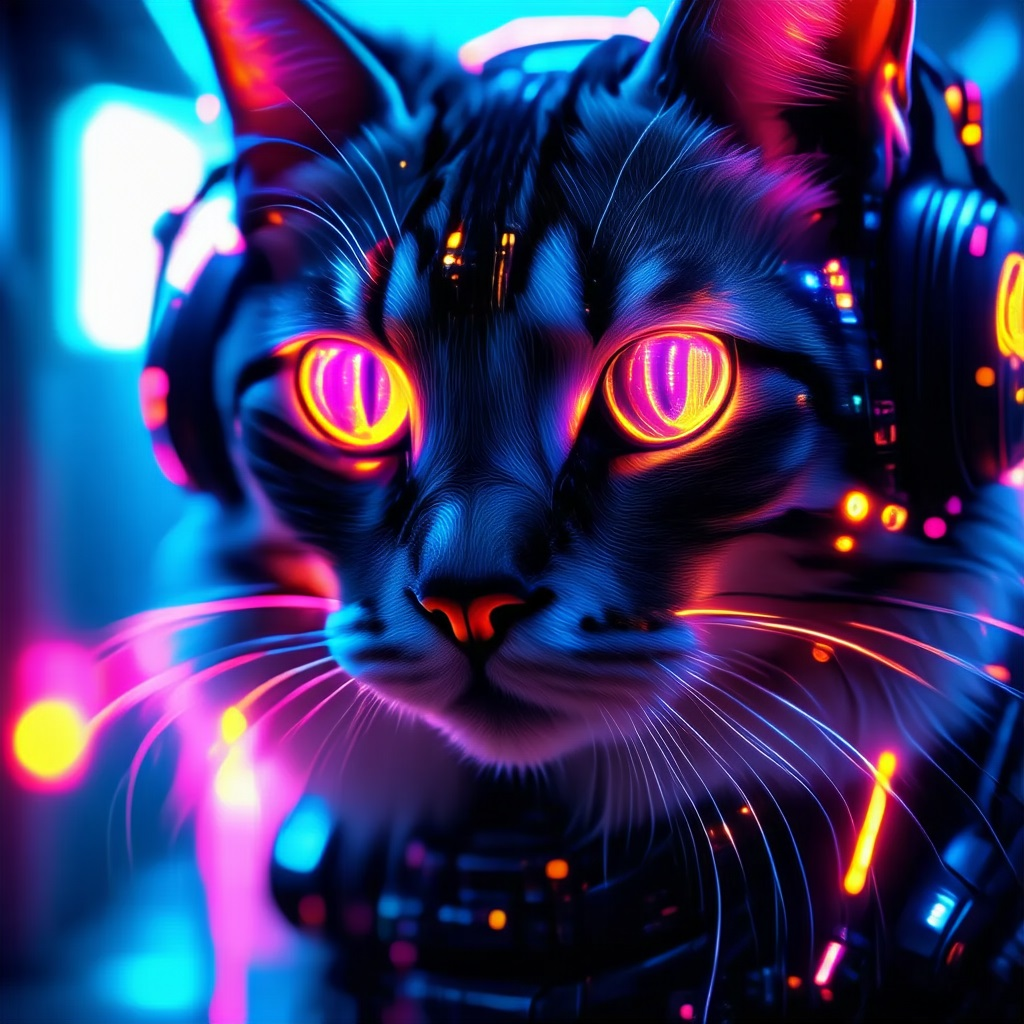
\includegraphics[width=0.19\linewidth]{figures/sec05_experiments/foundational_jz_fig/144000_jpg_prompt13_img2.jpg} &
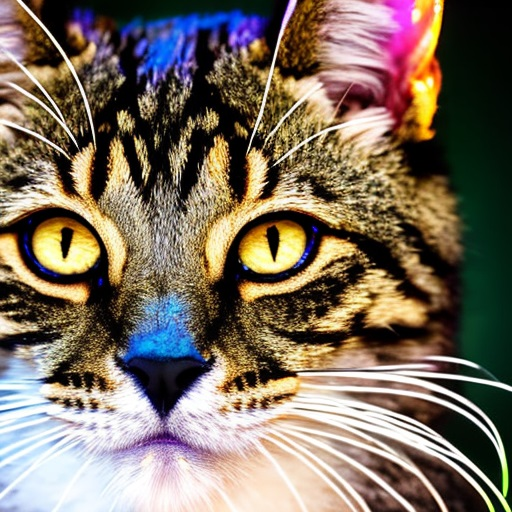
\includegraphics[width=0.19\linewidth]{figures/sec05_experiments/foundational_sd_fig/013_20260309_193648.jpg} &

\includegraphics[width=0.19\linewidth]{figures/sec05_experiments/SDV21/image_012.jpg} &

\includegraphics[width=0.19\linewidth]{figures/sec05_experiments/SDxl/image_012.jpg} &
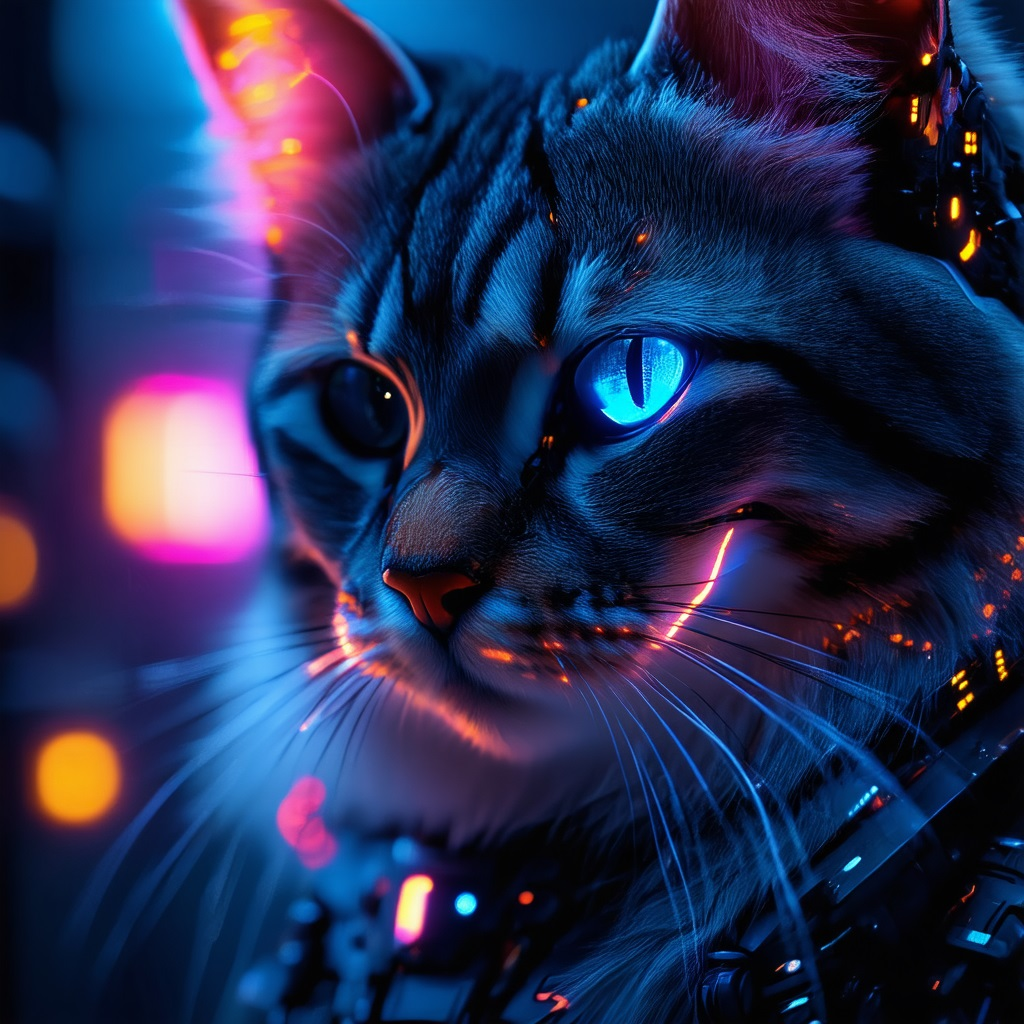
\includegraphics[width=0.19\linewidth]{figures/sec05_experiments/SD35/image_012.jpg} \\
\multicolumn{5}{p{0.98\linewidth}}{\centering\footnotesize (e) A striking close-up portrait of a cyberpunk cat, highly detailed fur, glowing neon reflections in its eyes, cinematic lighting, bokeh background, 8k resolution, photorealistic.} \\[1pt]

\end{tabular}
\caption{Qualitative comparison of $1024\times1024$ images generated by our 28-step base model against the Stable Diffusion family (SD\,1.5, SD\,2.1, SDXL, SD\,3.5-L) across five diverse prompts. Despite its 0.385B parameter budget, JuZhou 1.0 consistently achieves competitive visual fidelity in lighting, texture, and compositional structure.}
\label{fig:foundational_fig}
\end{figure}

\subsubsection{Foundational Generation Quality}
We assess overall visual fidelity by comparing images generated by our 28-step base model against Stable Diffusion variants (v1.5, v2.1, XL, and 3.5-L) using identical English prompts.
As illustrated in Fig.~\ref{fig:foundational_fig}, despite its significantly smaller parameter count, JuZhou 1.0 produces images with complex lighting, fine-grained textures, and strong 3D structural consistency, achieving perceptual quality comparable to---and occasionally surpassing---that of considerably larger models.

\begin{figure}[htbp]
\centering
\setlength{\tabcolsep}{1.2pt}
\renewcommand{\arraystretch}{1.05}

\newcommand{\cmpimg}[1]{%
\includegraphics[width=0.194\linewidth,height=0.118\textheight,keepaspectratio]{#1}
}

\begin{tabular}{ccccc}
\textbf{Orig. 4 steps} & \textbf{Orig. 8 steps} & \textbf{Orig. 16 steps} & \textbf{Orig. 28 steps} & \textbf{Ours (4 steps)} \\[3pt]

\cmpimg{figures/sec05_experiments/4steps/144000_jpg_prompt1_img3.jpg} &
\cmpimg{figures/sec05_experiments/8steps/144000_jpg_prompt1_img4.jpg} &
\cmpimg{figures/sec05_experiments/16steps/144000_jpg_prompt1_img2.jpg} &
\cmpimg{figures/sec05_experiments/28vs4_28/144000_jpg_prompt1_img2.jpg} &
\cmpimg{figures/sec05_experiments/28vs4_4/dmd_64000_jpg_prompt1_img2.jpg} \\
\multicolumn{5}{c}{\parbox{0.96\linewidth}{\centering\footnotesize (a) cinematic portrait of a medieval knight wearing detailed silver armor, dramatic lighting, ultra realistic, 8k.}} \\[7pt]

\cmpimg{figures/sec05_experiments/4steps/144000_jpg_prompt2_img1.jpg} &
\cmpimg{figures/sec05_experiments/8steps/144000_jpg_prompt2_img1.jpg} &
\cmpimg{figures/sec05_experiments/16steps/144000_jpg_prompt2_img1.jpg} &
\cmpimg{figures/sec05_experiments/28vs4_28/144000_jpg_prompt4_img2.jpg} &
\cmpimg{figures/sec05_experiments/28vs4_4/dmd_64000_jpg_prompt4_img2.jpg} \\
\multicolumn{5}{c}{\parbox{0.96\linewidth}{\centering\footnotesize (b) fashion photography of a futuristic cyberpunk woman with neon lights, studio lighting, high detail.}} \\[7pt]

\cmpimg{figures/sec05_experiments/4steps/144000_jpg_prompt3_img1.jpg} &
\cmpimg{figures/sec05_experiments/8steps/144000_jpg_prompt3_img1.jpg} &
\cmpimg{figures/sec05_experiments/16steps/144000_jpg_prompt3_img1.jpg} &
\cmpimg{figures/sec05_experiments/28vs4_28/144000_jpg_prompt12_img2.jpg} &
\cmpimg{figures/sec05_experiments/28vs4_4/dmd_64000_jpg_prompt12_img2.jpg} \\
\multicolumn{5}{c}{\parbox{0.96\linewidth}{\centering\footnotesize (c) a massive futuristic spaceship docking at a space station, cinematic science fiction scene.}} \\[7pt]

\cmpimg{figures/sec05_experiments/4steps/144000_jpg_prompt4_img3.jpg} &
\cmpimg{figures/sec05_experiments/8steps/144000_jpg_prompt4_img3.jpg} &
\cmpimg{figures/sec05_experiments/16steps/144000_jpg_prompt4_img3.jpg} &
\cmpimg{figures/sec05_experiments/28vs4_28/144000_jpg_prompt15_img3.jpg} &
\cmpimg{figures/sec05_experiments/28vs4_4/dmd_64000_jpg_prompt15_img3.jpg} \\
\multicolumn{5}{c}{\parbox{0.96\linewidth}{\centering\footnotesize (d) a glass sculpture shaped like a swan, illuminated by colorful lights, ultra detailed.}} \\[7pt]

\cmpimg{figures/sec05_experiments/28vs4_e/e_0004.jpg} &
\cmpimg{figures/sec05_experiments/28vs4_e/e_0008.jpg} &
\cmpimg{figures/sec05_experiments/28vs4_e/e_0016.jpg} &
\cmpimg{figures/sec05_experiments/28vs4_e/e_0028.jpg} &
\cmpimg{figures/sec05_experiments/28vs4_e/e_dmd_4.jpg} \\
\multicolumn{5}{c}{\parbox{0.96\linewidth}{\centering\footnotesize (e) A majestic misty forest at dawn, volumetric god rays piercing through dense canopy, ethereal atmosphere, cinematic photography.}} \\[4pt]

\end{tabular}

% \caption{Comprehensive visual comparison of generation quality under different sampling step settings. Each row presents a representative prompt, while the columns correspond to images generated by the original model with 4, 8, 16, and 28 sampling steps, respectively,
% together with the result produced by our distilled 4-step model. As the number of sampling steps decreases, the original model exhibits progressive deterioration in quality, including structural instability, loss of fine-grained details, and reduced semantic fidelity.
% In contrast, our distilled model consistently produces images visually comparable to those generated by the original 28-step model, demonstrating that a $7\times$ reduction in sampling steps can be achieved with little perceptual degradation.}
\caption{Qualitative visual comparison under different sampling step settings. Each row presents a representative prompt, and the columns show images generated by the original 28-step base model when sampled with 4, 8, 16, and 28 steps, followed by the result of our distilled 4-step model. When the undistilled base model is directly evaluated with fewer sampling steps, image quality tends to degrade, with visible artifacts such as structural instability, loss of fine-grained details, and reduced semantic fidelity. In contrast, the distilled 4-step model recovers much of the visual quality of the original 28-step model in these examples, showing that DMD2 distillation enables a $7\times$ reduction in sampling steps with limited perceptual degradation.}
\label{fig:28vs4}
\end{figure}

\subsubsection{Distillation Efficacy and Acceleration}
Fig.~\ref{fig:28vs4} illustrates the effectiveness of our DMD2 distillation strategy.
While the non-distilled model suffers from structural collapse at lower inference steps (4, 8, and 16 steps), our 4-step distilled model maintains visual fidelity nearly identical to the 28-step baseline.
This $7\times$ acceleration introduces virtually no perceptual degradation, yielding an optimal efficiency-fidelity trade-off for on-device deployment~\cite{yin2024improved_dmd,luo2023lcm}.

